\section{Introduction}

Given a binary relation $R$ such that is:
\begin{itemize}
    \item Reflexive: $a R a$
    \item Symmetric: $a R b \Rightarrow b R a$
    \item Transitive: $a R b \land b R c \Rightarrow a R c$
\end{itemize}

we say that $R$ provides a partition $\Pi$ of $A$ into disjoint equivalence classes. That is, $\Pi = \{A_1, \ldots, A_k\}$ is defined as follows:

\begin{itemize}
    \item $\forall A_i, A_j \in \Pi, A_i \cap A_j = \emptyset \iff A_i \neq A_j$
    \item $A = \bigcup\limits_{i = 1}^{k} A_i$
    \item $a \equiv b \iff a,b \in A_i$ for some $A_i \in \Pi$.
\end{itemize}


Such idea was used in Computer Science by Galler and Fisher\cite{galler1964improved} as the \textbf{union-find data structure} which is a data structure that stores partition of a set into disjoint sets. In particular \textbf{union find} consist of two main operation:

\begin{itemize}
    \item Find Operation: Given two elements $a,b \in A$ determine if $\exists A_i \in \Pi$ s.t $a,b \in A_i$.
    \item Union Operation: Given two elements $a \in A_i$ and $b \in A_j$, \textit{merge} $A_i$ and $A_j$. That is, the result of this operation to the partition $\Pi$ will be a new partition $\Pi'$ such that $\Pi' = (\Pi \setminus \{A_i, A_j\}) \cup (A_i \cup A_j)$.
\end{itemize}

\section{Implementation}
From now on we are going to assume that our set $A$ is defined as $\{0, \ldots, n-1\}$ (and if it is not the case we can use a dictionary to map elements from $A$ to that range).

\subsection{Representation of the partition}
Since every subset defines an equivalence class, it is equivalent to represent each \( A_i \subseteq A \) with a single element \( r_i \in A_i \), called the \textit{representative} of \( A_i \). Every other element of \( A_i \) is related to \( r_i \) by the properties of the previously defined binary relation.  That is why a union-find data structure consists of an array \( v[0:n-1] \), where each element \( i \in A \) either points to another element \( j \in A \) belonging to the same class (i.e., \( v[i] = j \)) or is the representative of a class and is \textit{marked specially} (in a few lines we are going to define what \textit{marked specially} is).  

For instance, Figure \ref{fig:example} provides an example of a union-find structure representing the partition \( \Pi = \{ \{0,1,2,3\}, \{4,5,6\} \} \). In this example, the class \( \{0,1,2,3\} \) has \( 1 \) as its representative (hence, its position is marked with a special symbol). Elements \( 0 \) and \( 3 \) point to the representative (indicated by the fact that both positions in the array contain \( 1 \)), while element \( 2 \) points to element \( 0 \), even though \( 0 \) is not the representative.  

Although our implementation will consist of an array, the tree representation in the figure will help in understanding the union-find structure. Since we are representing a directed tree, we know that there is always a unique path from any element to the representative. As we move along this path, we will eventually reach the representative.

\begin{figure}
    \centering
    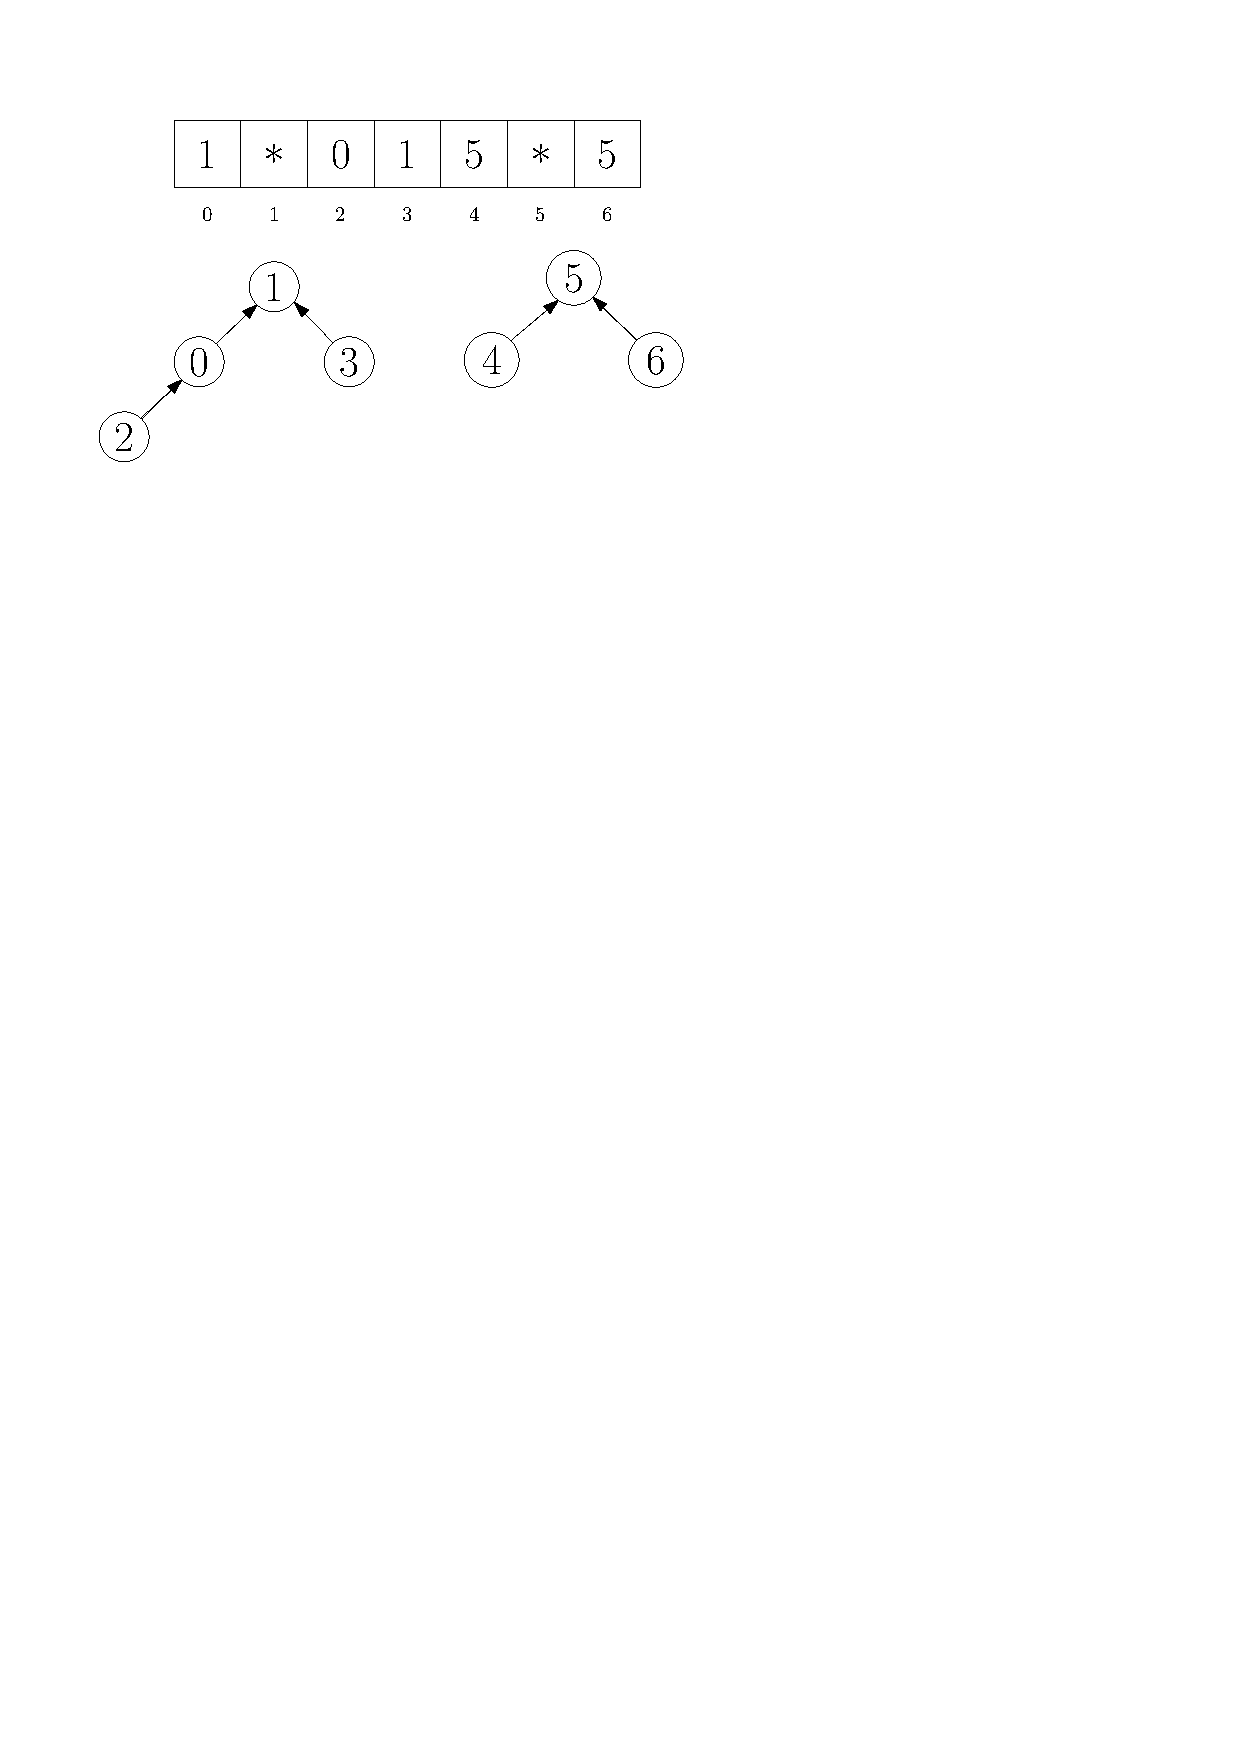
\includegraphics[scale=0.75]{images/ufExample.pdf}
    \caption{An example of a Union-Find with partition $\Pi = \{ \{0,1,2,3\}, \{4,5,6\}\}$}
    \label{fig:example}
\end{figure}

When defining how to represent the representative of a class, there are three natural ways to do so:

\begin{itemize}
    \item A representative $i \in A$ of some class can be represented by its own number (i.e., $v[i] = i$). We can identify such an element as the representative of a class because representatives are marked by their own position in the array. For instance, in the example of Figure \ref{fig:example}, we can mark element $1$ with $v[1] = 1$ and element $5$ with $v[5] = 5$.
    
    \item A representative $i \in A$ of some class can be represented by the size of the tree it holds. Although the size of a tree is a natural number, we can use negative numbers to indicate that position $i$ is the representative of a class, with the negative value representing the size (i.e., $v[i] = -\text{size}$). For instance, in the example of Figure \ref{fig:example}, we can mark element $1$ with $v[1] = -4$ and element $5$ with $v[5] = -3$.
    
    \item A representative $i \in A$ of some class can be represented by the rank of the tree it holds (again, using negative numbers). The rank of a tree is related to its height (later, we will see that the rank does not always correspond to the exact height, but we will use it as an upper bound). For instance, in the example of Figure \ref{fig:example}, we can mark element $1$ with $v[1] = -2$ and element $5$ with $v[5] = -1$.
\end{itemize}

\subsection{Find Operation}
Let us first implement the \textit{find} operation, which consists of finding, for a given element \( i \in A \), the representative \( r_i \) of the class to which \( i \) belongs.

From what we know about union-find, every element in a certain class will either point to the representative of the class or to another element that lies on the path between the representative and itself. Since we are representing a directed tree, we will eventually reach the representative.

Thus, our algorithm will consist of traversing this path until we reach the representative. Algorithm \ref{alg:find} gives a simple description of how we can do that.

\begin{algorithm}
    \caption{Find Operation}\label{alg:find}
    \begin{algorithmic}
        \Function{Find}{$v$, $i$}
        \State $r_i \gets i$
        \While {$\neg isRepresentative(v[r_i])$}
        \State $r_i \gets v[r_i]$
        \EndWhile
        \State \Return $r_i$
        \EndFunction
    \end{algorithmic}
\end{algorithm}

One can check if an element is the representative of a class or not in $\Theta(1)$ time, but the implementation will depend on how the representative is defined. Still, it requires only one comparison.

The cost of the find operation depends on the height of the tree that represents the class. One might assume that, in the worst case, we are going to have a single unbalanced tree, and in such a case, the cost of the find operation is $O(n)$, which holds true if no heuristics are used in order to rearrange the tree. So let us apply heuristics during the find execution (switching some pointers) in order to speed up future calls of that operation (which is called \textit{path compression}). 

\subsubsection{Full path compresion}
The idea behind this heuristic is to traverse the path from \(i\) to \(r_i\) twice: once to determine \(r_i\) and once more to make every node within the path point to \(r_i\). Although this doubles the cost of the find operation, we expect that a future find operation on the same class will be faster than usual. Algorithm \ref{alg:findPathComp} provides an implementation of such heuristic.

\begin{algorithm}
    \caption{Find operation with path compression}\label{alg:findPathComp}
    \begin{algorithmic}
        \Function{Find}{$v$, $i$}
        \If{$isRepresentative(v[i])$}
        \State \Return $i$
        \Else
        \State $v[i] = Find(v,v[i])$
        \State \Return $v[i]$
        \EndIf
        \EndFunction
    \end{algorithmic}
\end{algorithm}

\subsubsection{Path Splitting}
In order to not traverse twice the path we can make that every node points to its grandparent (except if they do not have). Although the tree will not be as balanced as with the previous heuristic we are not traversing twice the path which might impact in the performance of the operation. Algorithm \ref{alg:findPathSplt} provides an implementation of such heuristic.


\begin{algorithm}
    \caption{Find operation with path splitting}\label{alg:findPathSplt}
    \begin{algorithmic}
        \Function{Find}{$v$, $i$}
        \If{$isRepresentative(v[i])$}
        \State \Return $i$
        \EndIf
        \State $i_1 \gets i$
        \State $i_2 \gets v[i_1]$
        \While{$\neg isRepresentative(v[i_2])$}
        \State $v[i_1] = v[i_2]$
        \State $i_1 = i_2$
        \State $i_2 = v[i_2]$
        \EndWhile
        \State \Return $i_2$
        \EndFunction
    \end{algorithmic}
\end{algorithm}


\subsubsection{Path Halving}
We can also make that every other node points to its grand-parent. Algorithm \ref{alg:findPathHalv} provides an implementation of such heuristic.


\begin{algorithm}
    \caption{Find operation with path splitting}\label{alg:findPathHalv}
    \begin{algorithmic}
        \Function{Find}{$v$, $i$}
        \If{$isRepresentative(v[i])$}
        \State \Return $i$
        \EndIf
        \State $i_1 \gets i$
        \State $i_2 \gets v[i_1]$
        \State $setParent \gets true$
        \While{$\neg isRepresentative(v[i_2])$}
        \If{$setParent$}
        \State $v[i_1] = v[i_2]$
        \EndIf
        \State $setParent \gets \neg setParent$
        \State $i_1 = i_2$
        \State $i_2 = v[i_2]$
        \EndWhile
        \State \Return $i_2$
        \EndFunction
    \end{algorithmic}
\end{algorithm}
